\documentclass[journal]{IEEEtran}
%\IEEEoverridecommandlockouts
% The preceding line is only needed to identify funding in the first footnote. If that is unneeded, please comment it out.

% listings package for code blocks
\usepackage{listings}
\usepackage{xcolor}
\usepackage{cite}
\usepackage{verbatim}
\usepackage{graphicx}
\usepackage{parskip}

\begin{document}

% overfull \hbox .. too wide 
\setlength{\emergencystretch}{12pt}
%\setlength{\parskip}{0pt} % 1ex plus 0.5ex minus 0.2ex}
\setlength{\parindent}{10pt}

\definecolor{codegreen}{rgb}{0,0.6,0}
\definecolor{codegray}{rgb}{0.5,0.5,0.5}
\definecolor{codepurple}{rgb}{0.58,0,0.82}
\definecolor{backcolour}{rgb}{0.95,0.95,0.92}

\lstdefinestyle{mystyle}{
    backgroundcolor=\color{backcolour},   
    commentstyle=\color{codegreen},
    keywordstyle=\color{magenta},
    numberstyle=\tiny\color{codegray},
    stringstyle=\color{codepurple},
    basicstyle=\ttfamily,
    breakatwhitespace=false,         
    breaklines=true,      
    postbreak=\mbox{\textcolor{red}{$\hookrightarrow$}\space},           
    captionpos=b,
}

\lstset{style=mystyle}

\title{Investigating Decision Trees}

\author{
\IEEEauthorblockN{Lillian Mueller}
\IEEEauthorblockA{lmuelle1@umd.edu}
\\
\IEEEauthorblockN{Regina Hong}
\IEEEauthorblockA{rhong@umd.edu}
}

\maketitle

\begin{abstract}
\label{log:abstract}
This report explored the development of a decision tree model to classify Iris species. In a decision tree model, the target attribute is chosen and the data is broken down, or segmented, into groups based on information gain and entropy of the dataset or group. We investigated how manipulating the purity measure criterion affects the overall performance of the decision tree. For this dataset, we found that deriving information gain via entropy versus Gini index has largely the same outcome.
\end{abstract}

\section{Introduction}

In the decision tree model creation process, attributes are selected based on information gain and the purity of the segments purity which can be measured via the entropy of the group or using the Gini index. In the case of classification, a segment\textquotesingle s purity measures how closely the data fits into a single category (entropy) or the likelihood that a sample belongs to a single category (Gini index) \cite{b2}. This calculation helps evaluate the effectiveness of each node and how well it will perform \cite{b1}. 

This investigation will demonstrate how manipulating supervised segmentation and tuning the purity measurements can increase accuracy and performance of the decision tree model. Along the way, we will be experimenting with the information gain and purity measurements to observe the performance of the decision tree model.

The focal dataset is the Iris dataset, supplied by the \lstinline{scikitlearn} library. This dataset contains four measurements for each Iris flower: sepal length, sepal width, petal length, and petal width. Alongside these features, the classification of each Iris flower is given; the flower is classified as setosa, versicolor,
or virginica. 


Section II describes methodology followed during the course of this study. Section III contains the results of the model. Finally, a brief discussion of the results and future applications is offered in Section IV.

\section{Methodology}
Several Python packages were utilized in order to view the Iris dataset, build a Decision Tree model, and test the model. The majority of the modeling and analysis comes from various modules stemming from the \lstinline{scikit-learn} (sklearn) package.

\begin{lstlisting}[language=Python, caption=Libraries used for this assignment.]
from sklearn.datasets import load_iris
from sklearn.tree import DecisionTreeClassifier
from sklearn import tree, preprocessing
from sklearn.model_selection import train_test_split
from sklearn.metrics import accuracy_score, r2_score
import pandas as pd 
import numpy as np
\end{lstlisting}

First, the Iris dataset was loaded as an \lstinline{sklearn.utils.Bunch} object via the \lstinline{load_iris()} function, which was assigned to \lstinline{iris_data}. This object is similar to a Python dictionary. To make the data easier to read, the pandas package was imported and used to transform said dictionary into the \lstinline{df_iris} dataframe, where the data parameter was set as the data attribute of the dataset and the columns parameter as the \lstinline{feature_names} attribute. A new column called “class” was added to this dataframe which contains the \lstinline{target} variable of the Iris dataset; this is the class of the Iris plant \textemdash setosa, versicolor, or virginica. Since the \lstinline{target} attribute contains an array with values from 0-2, the \lstinline{.replace} function was used to map these numerical values to their corresponding classifications: setosa for \lstinline{0}, versicolor for \lstinline{1}, and virginica for \lstinline{2}. 

With \lstinline{df_iris} ready for processing, the next step was to build an initial Decision Tree. To do this, the \lstinline{DecisionTreeClassifier()} function from \lstinline{sklearn} was used with default parameters.

\begin{lstlisting}[language=Python, caption=Building the Decision Tree]
dt_model = tree.DecisionTreeClassifier()
predictors, target = iris_data.data, iris_data.target
dt_model.fit(predictors, target)
\end{lstlisting}

Then, the actual tree diagram was created using \lstinline{graphviz}, with \lstinline{feature_names=iris_data.feature_names} and \lstinline{class_names=iris_data.target_names} so that the resulting file contained the feature and class names for ease of reading. 

The nodes of the Decision Tree diagram were compared to the process that was run in a referenced model in Excel. Using petal length as the parent node, it should be noted that the Decision Tree reflected the same splitting process as the Excel model, choosing the same values.

This same Decision Tree making process was run again, this time specifying the \lstinline{criterion} parameter of \lstinline{DecisionTreeClassifier()} function as \lstinline{criterion='entropy'} to see how using Shannon entropy instead of Gini impurity changes the way the Decision Tree is created. Differences between the two Decision Trees are reviewed in the results section.

Since the Iris dataset is relatively small, two parameters in the \lstinline{DecisionTreeClassifier()} function were independently changed to determine how the tree model changes. The first is \lstinline{max_depth}, which controls the size of the tree by limiting the number of levels. Since each internal node requires at minimum 2 child nodes, setting this value to a smaller number stops additional splits that may lead to overfitting. The second parameter is \lstinline{min_samples_split}; setting a value greater than the default of 2 ensures that splits will not happen when a node only has 2 samples, which may also reduce the possibility of overfitting. 

Next, the Iris dataset was split into a test group and train group, where the train group underwent the Decision Tree Classification modeling process and the test group was then used in the resulting model. To split the data into those two groups, the \lstinline{train_test_split} function was imported from the \lstinline{sklearn.model_selection} module with the \lstinline{test_size} parameter set to 0.33 so that around \(\frac{1}{3}\) of the data is set aside for testing. 

After the Decision Tree model was fitted to the training data, an accuracy score was used to see how well the results from the test data matched with actual data. To do this, the \lstinline{accuracy_score} function was imported from \lstinline{sklearn.metrics} module, setting the \lstinline{y_true} parameter to data from the original dataset and \lstinline{y_pred} to data produced from the classifier. 

The test and train process was repeated again with 20\% of the dataset reserved as test data and the other 80\% as training data. Once again, the accuracy scores of the train and test data were printed and observed. Additional iterations of this process used the same test/train data split (\(\frac{1}{3}\) to \(\frac{2}{3}\)) but this time also varied the \lstinline{max_depth} and \lstinline{criterion} parameters to see their effects on the accuracy of the train and test data.

\section{Results}

In this investigation, SKLearn\textquotesingle s DecisionTreeClassifier was used to create decision tree models for the Iris dataset. By manipulating the parameters for this class, we were able to develop different trees to classify the Iris data by species. The main parameter we focused on was the “criterion” parameter which allows the developer to change the function by which to measure quality of the splits in the dataset. The first function investigated was the Gini Impurity function. After each split, the method evaluates the likelihood a random sample in the group could be misclassified \cite{b2}. This means that the lower the Gini index, the better the split is as there is a low likelihood a sample will be misclassified. Figure~\ref{fig:dtGI} below shows a depiction of the tree derived from this method.

\begin{figure}[h!]
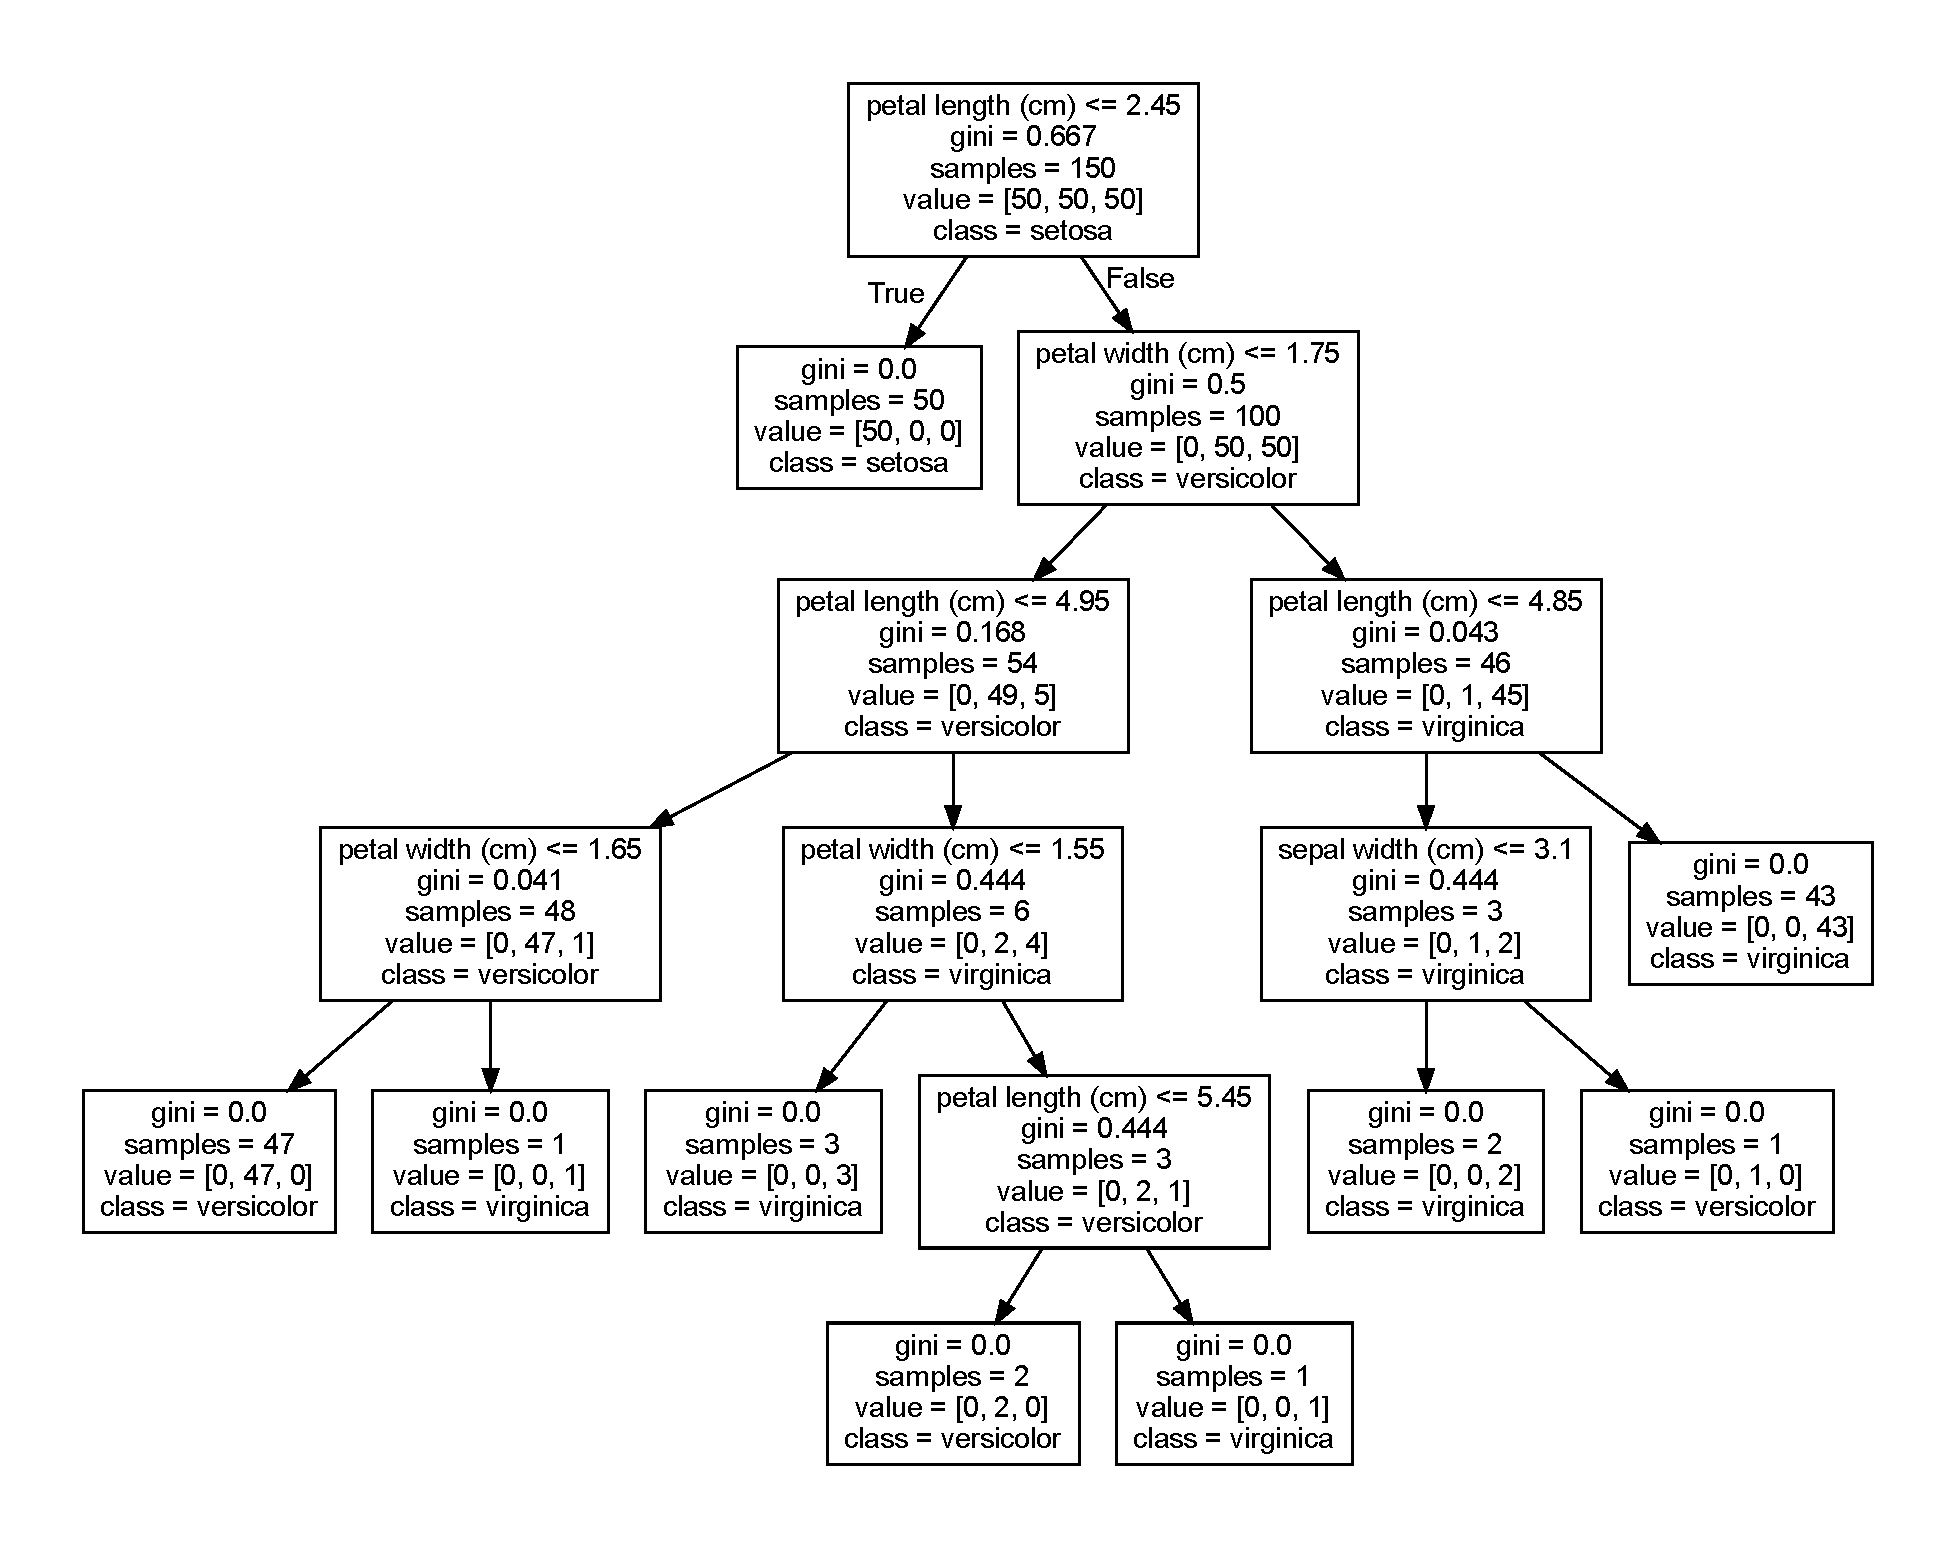
\includegraphics[scale=0.25]{iris.pdf}
\centering
\caption{Decision Tree Utilizing Gini Impurity Criterion}
\label{fig:dtGI}
\end{figure}

In this tree, each node shows the defining attribute, the Gini index value, the number of samples, the sample breakdown, and the favored class. Just looking at the tree, one can infer that the virginica and versicolor class of iris are difficult to tell apart as their attributes greatly overlap. While setosa can be classified within the first level of the tree, the others take up to 5 levels. To determine the accuracy of this model and evaluate its performance, 1000 models were developed using random training sets and the model accuracy was tested using the respective testing sets. The accuracy of the model using the Gini Impurity methods converged to 0.9451 and had an average r2 score of 0.916, as seen in Table~\ref{table:dtGI} below. For this dataset, these statistics prove that the Decision Tree model is effective in classifying Iris species. 

\begin{table}[h!]
\centering
\begin{tabular}{ c | c c c }
    Description & Train Data Accuracy & Test Data Accuracy & r2 Score \\ 
\hline
count & 1000.0    & 1000 & 1000  \\
mean  &    1.0    &    0.945100   &  0.915793 \\
std   &    0.0    &    0.028636   &  0.044914 \\
min   &    1.0    &    0.840000   &  0.750000 \\
25\%  &     1.0   &     0.920000  &   0.887892 \\
50\%  &     1.0   &     0.940000  &   0.916574 \\
75\%  &     1.0   &     0.960000  &   0.942824 \\
max   &   1.0     &   1.000000    & 1.000000
\end{tabular}
\caption{Statistics for Decision Tree utilizing Gini Impurity Criterion}
\label{table:dtGI}
\end{table}

The second function we investigated was entropy. This method evaluates the purity of the split by qualifying the disorder within the group. The more variability within the samples, the greater the entropy value for that node. The following is a depiction of the tree derived from this method along with its performance logistics. 

\begin{figure}[h!]
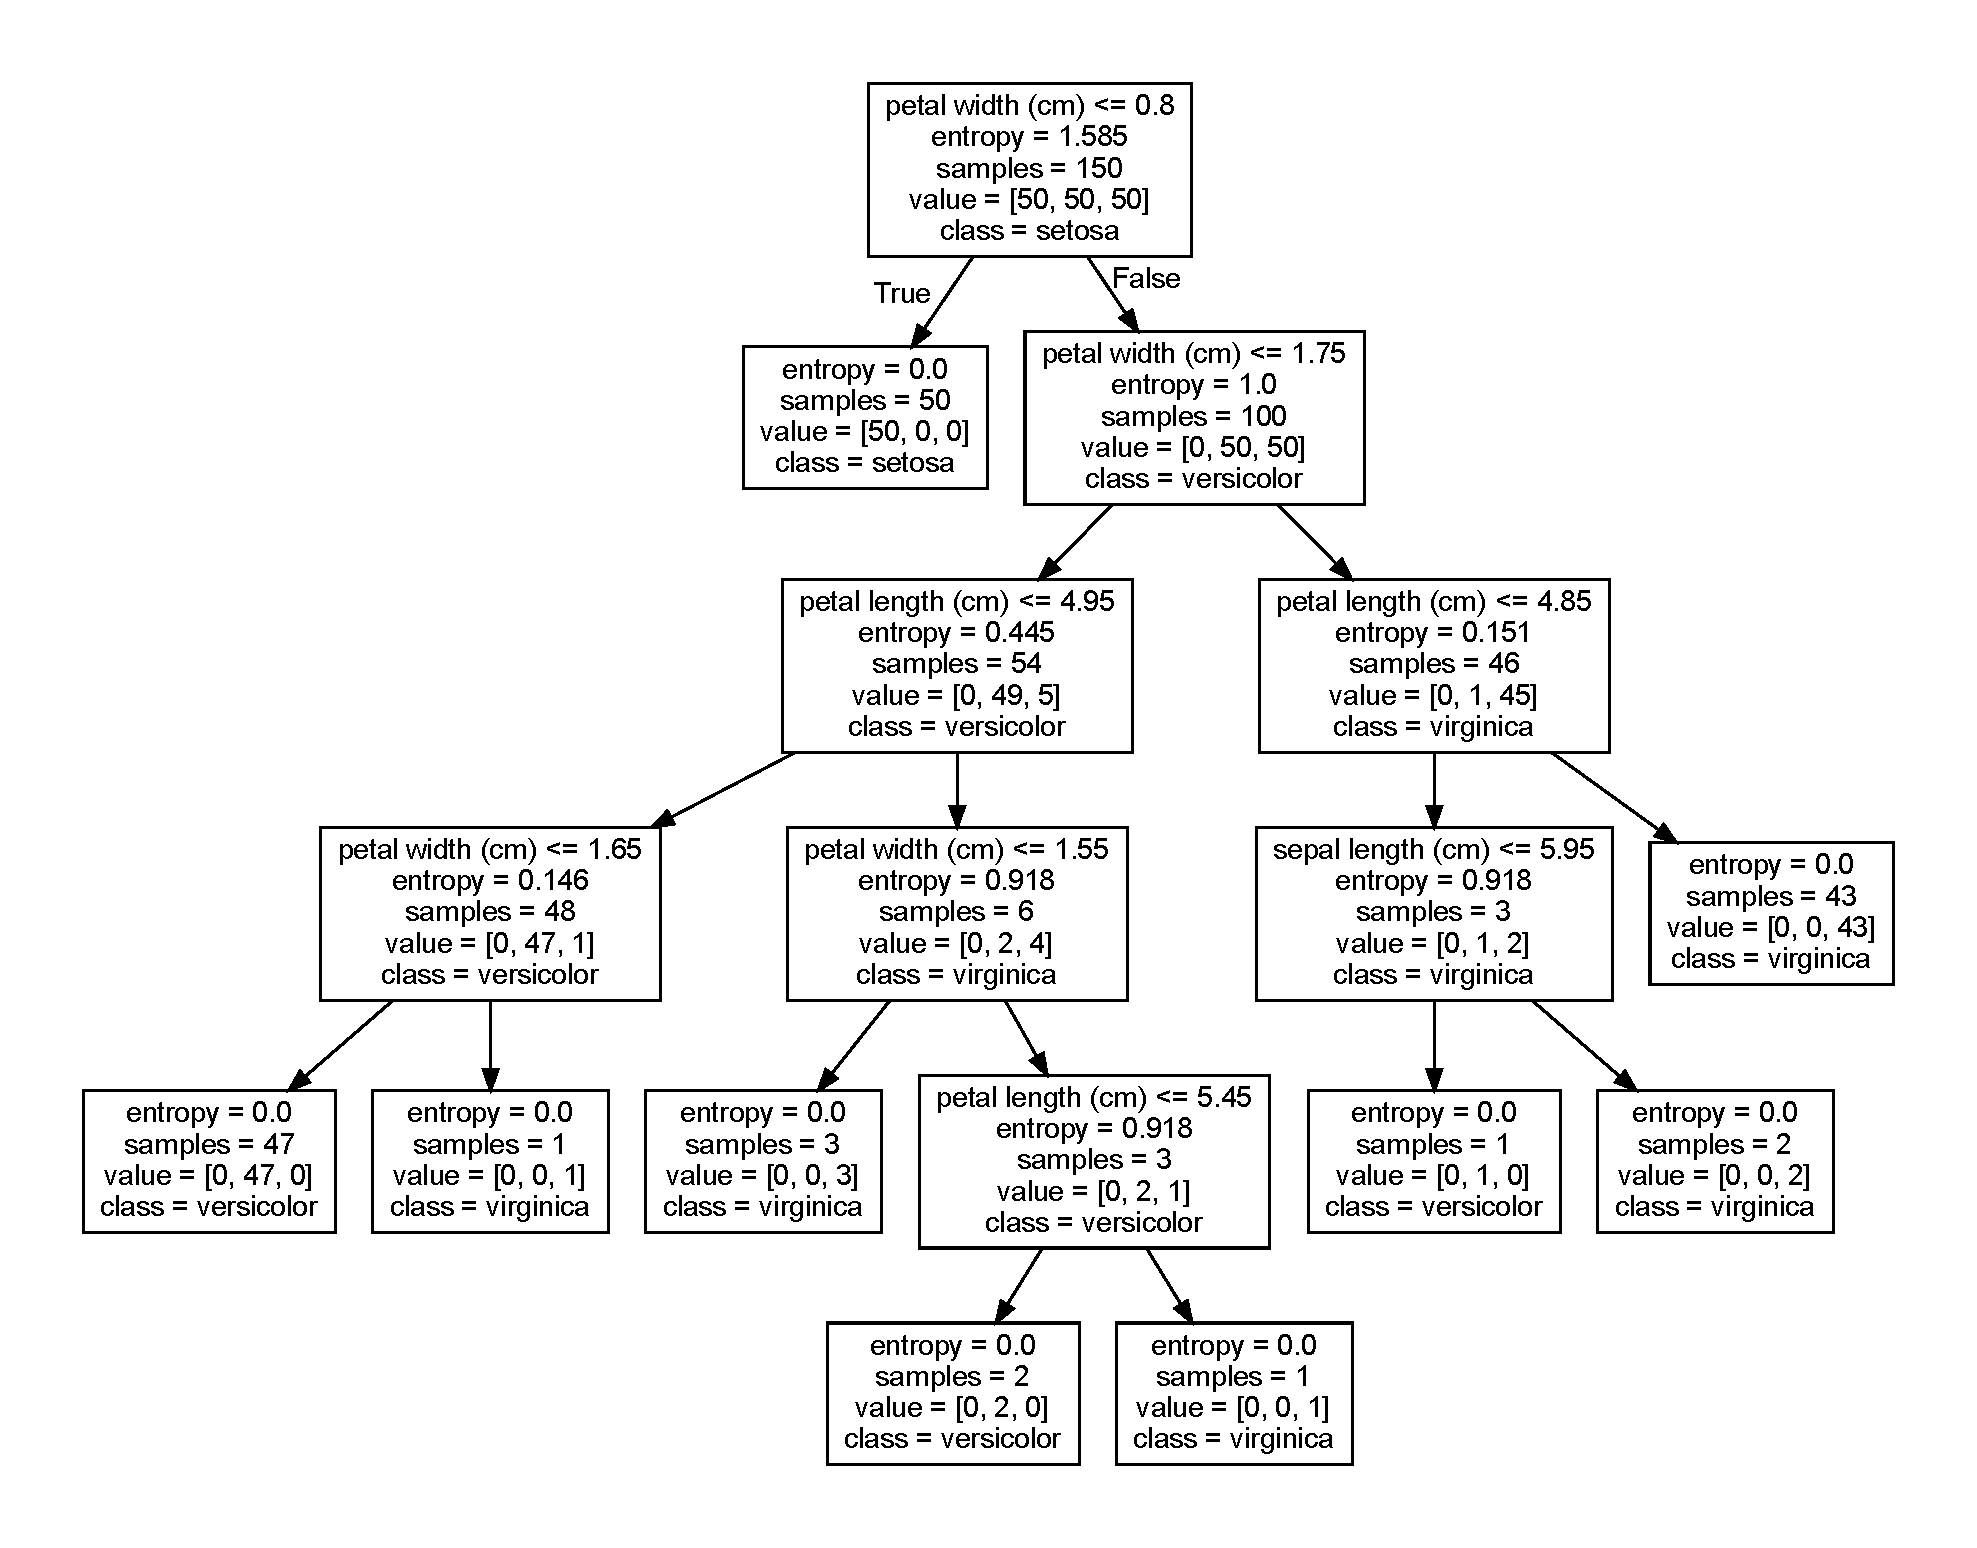
\includegraphics[scale=0.25]{iris2.pdf}
\centering
\caption{Decision Tree Utilizing Entropy Criterion}
\label{fig:dtEn}
\end{figure}

Each node in the tree shown in Figure~\ref{fig:dtEn} also shows similar values to the previous tree. However, rather than displaying the Gini index, the nodes show the entropy measurement at each split. Where Gini index values range from 0 to 0.5, entropy values range from 0 to 1. Additionally, there are some differences within the attributes chosen in each tree. For example, the root node in the first tree refers to petal length, whereas the second tree splits the root node by petal width. After running this model 1000 times over, the average accuracy converged to 0.9437 where the r2 score was 0.914. From this data, one can conclude that using entropy and the Gini index as a measure of purity is very similar, however the entropy metric is marginally better for this dataset.

\begin{table}[h!]
\centering
\begin{tabular}{ c | c c c }
    Description & Train Data Accuracy & Test Data Accuracy & r2 Score \\ 
\hline
count &              1000.0  &       1000 & 1000\\
mean  &                 1.0  &          0.943680 &    0.913660\\
std   &                 0.0  &          0.027291 &    0.043502\\
min   &                 1.0  &          0.780000 &    0.633333\\
25\%   &                 1.0  &          0.920000 &    0.886492\\
50\%   &                 1.0  &          0.940000 &    0.914237\\
75\%   &                 1.0  &          0.960000 &    0.942562\\
max   &                 1.0  &          1.000000 &    1.000000
\end{tabular}
\caption{Statistics for Decision Tree utilizing Entropy Criterion}
\label{table:dtEn}
\end{table}

While the accuracy of each model was very high, the accuracy of the model when applied to the training set was near 1.0. This could lead the analyst to hypothesize that the model may be overfitting the data. To combat this, an adjustment to the Decision Tree model was made so that the number of levels was constrained to 4. This newly altered model was then rerun. Figures~\ref{fig:dtGI4} and~\ref{fig:dtEn4} depict the resultant trees while Tables~\ref{table:dtGI4} and~\ref{table:dtEn4} present the breakdown of performance for the Gini Impurity and entropy methods, respectively. 

\begin{figure}[h!]
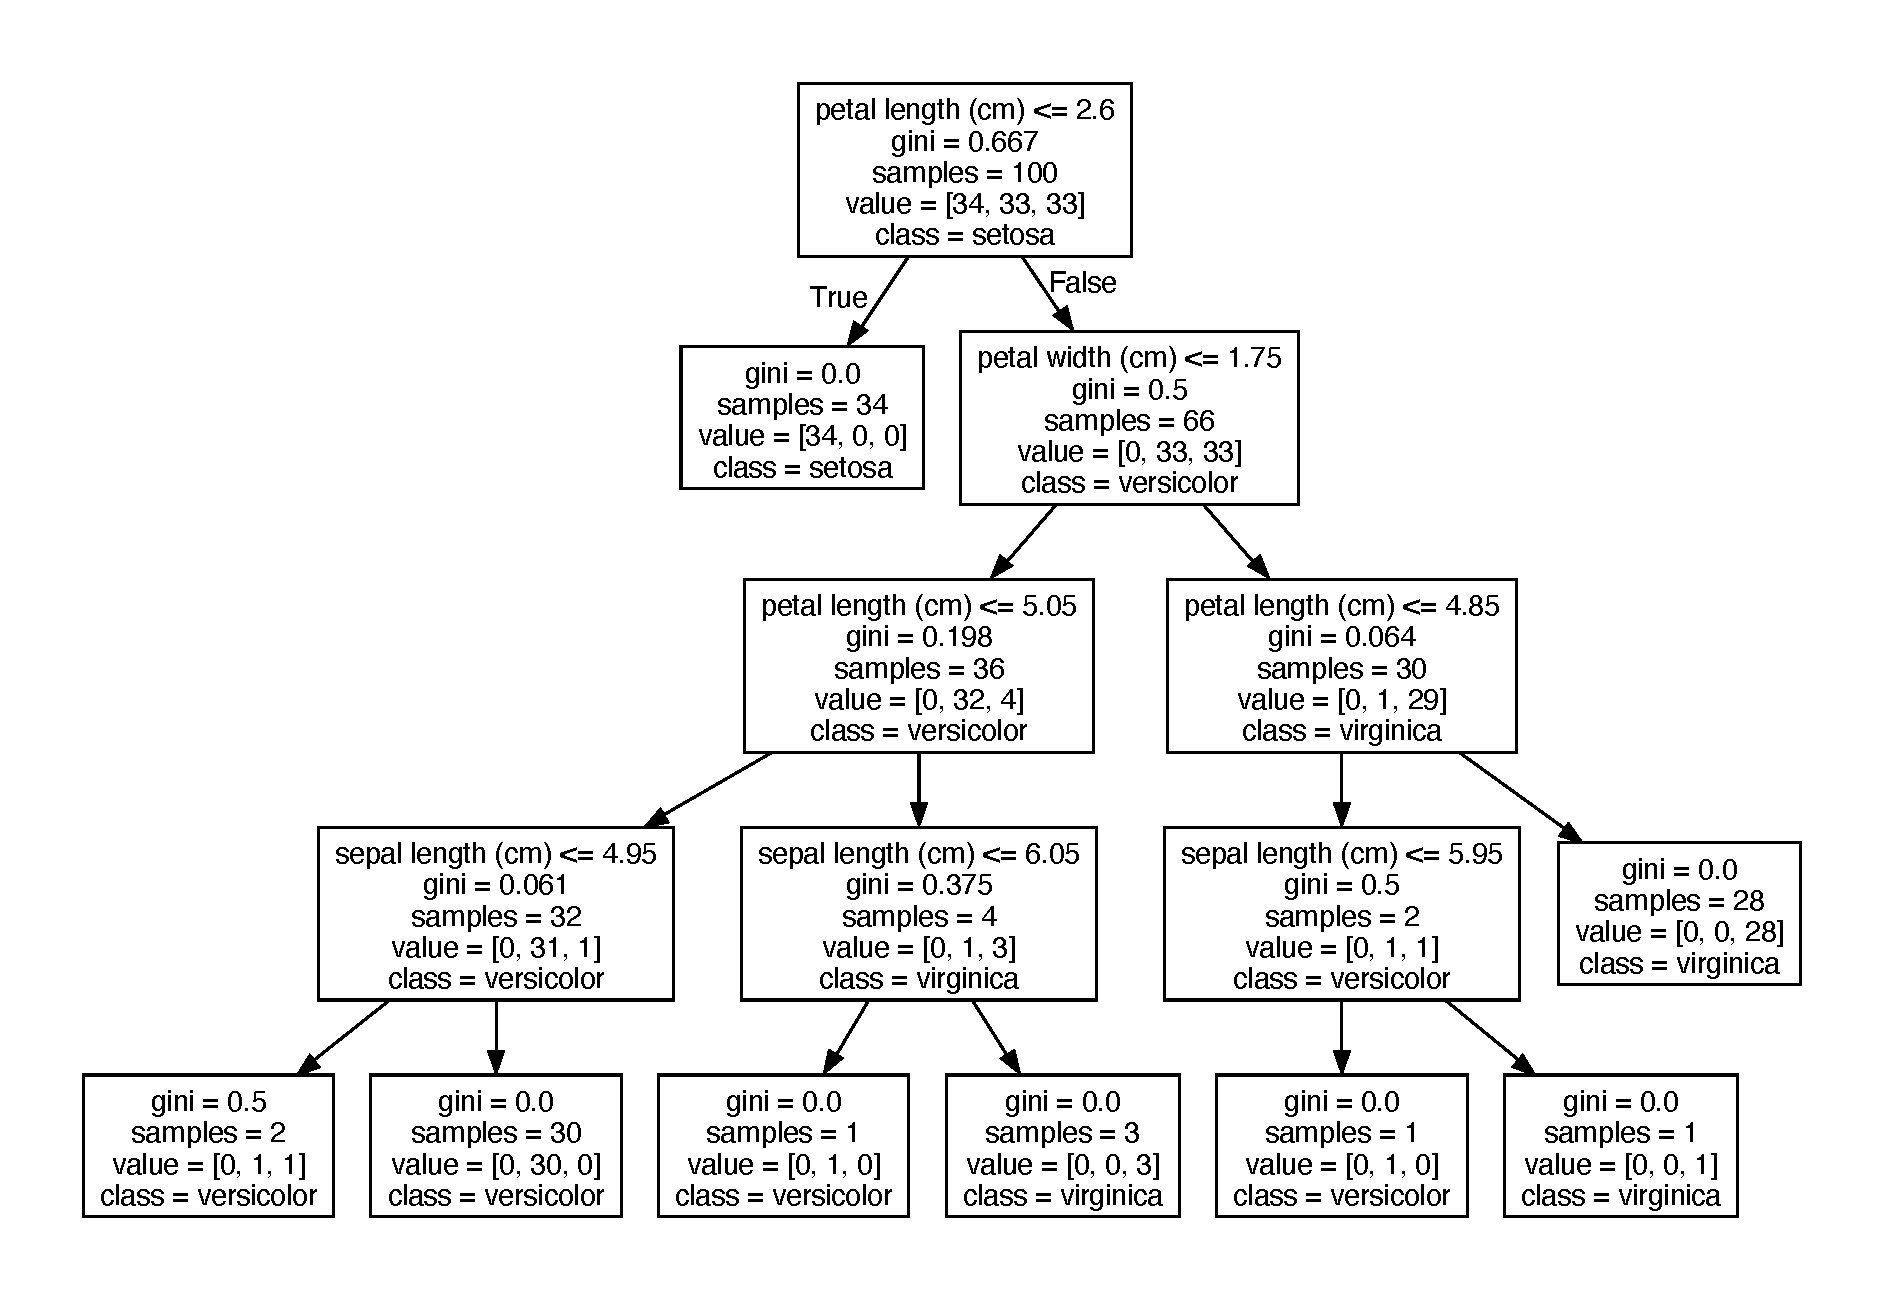
\includegraphics[scale=0.25]{iris-gini-4levels.pdf}
\centering
\caption{Decision Tree Utilizing Gini Impurity Criterion with 4 Levels}
\label{fig:dtGI4}
\end{figure}

\newpage


\begin{table}[h!]
\centering
\begin{tabular}{ c | c c c }
    Description & Train Data Accuracy & Test Data Accuracy & r2 Score \\ 
\hline
count     &     1000.000000     &    1000 & 1000\\
mean      &        0.992880     &       0.945540  &   0.916688\\
std       &        0.007494     &       0.027685  &   0.043817\\
min       &        0.970000     &       0.840000  &   0.678457\\
25\%      &         0.990000    &        0.920000 &    0.891068\\
50\%      &         0.990000    &        0.940000 &    0.916713\\
75\%      &         1.000000    &        0.960000 &    0.942562\\
max       &        1.000000     &       1.000000  &   1.000000
\end{tabular}
\caption{Statistics for Decision Tree Utilizing Gini Impurity Criterion (4 Levels}
\label{table:dtGI4}
\end{table}

\begin{figure}[h!]
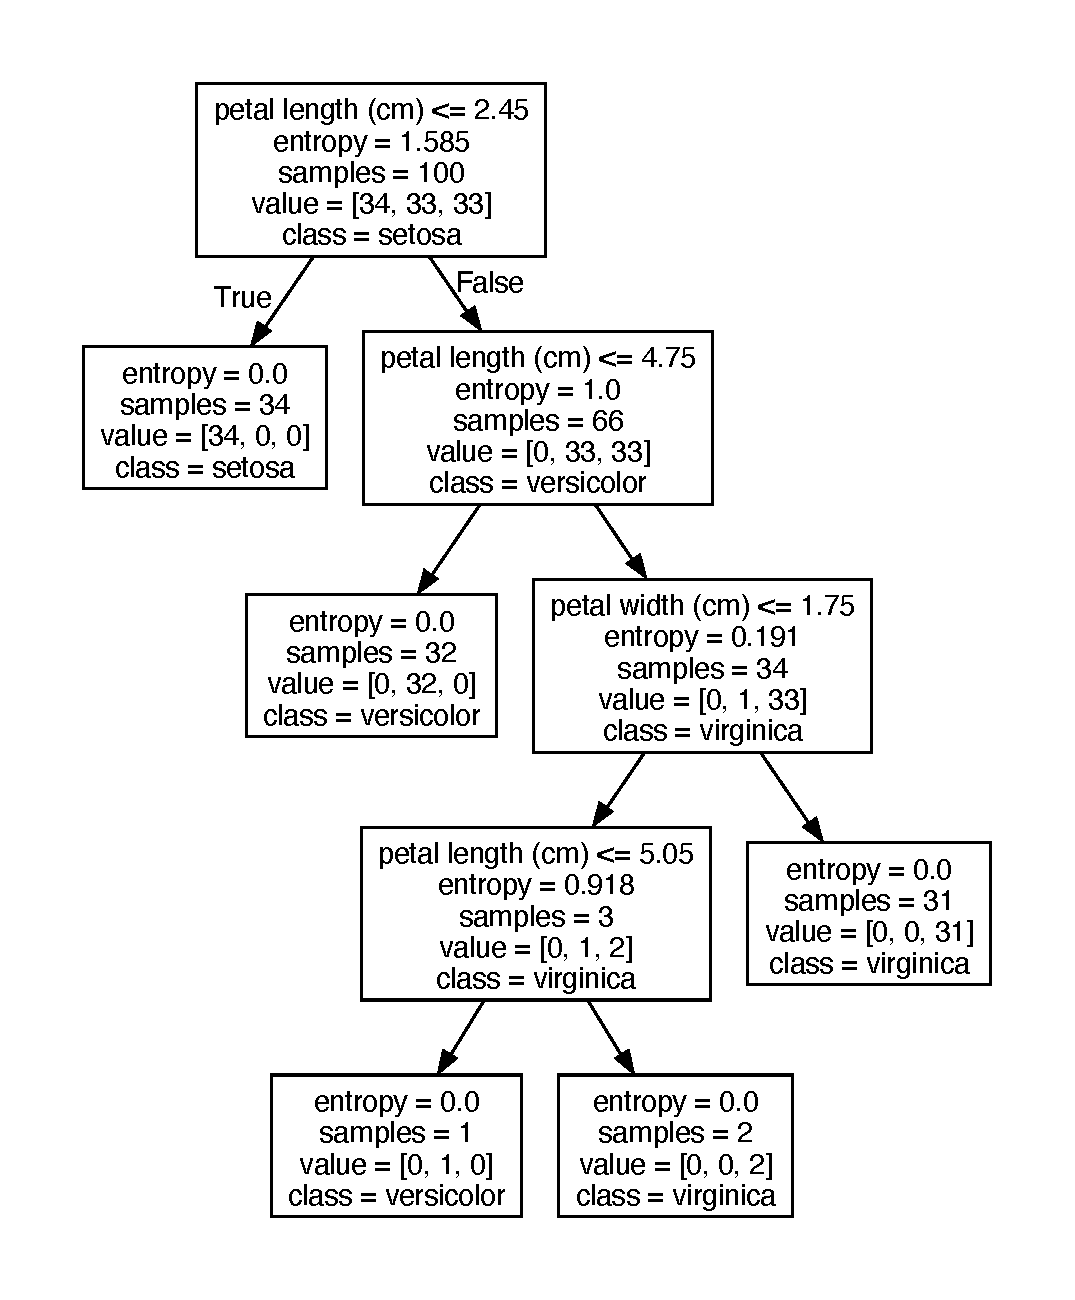
\includegraphics[scale=0.3]{iris-entropy-4levels.pdf}
\centering
\caption{Decision Tree Utilizing Entropy Criterion with 4 Levels}
\label{fig:dtEn4}
\end{figure}

\begin{table}[h!]
\centering
\begin{tabular}{ c | c c c }
    Description & Train Data Accuracy & Test Data Accuracy & r2 Score \\ 
\hline
count     &     1000.000000     &    1000  &1000\\
mean      &        0.992370    &        0.943140   &  0.912387\\
std       &        0.008953    &        0.027439   &  0.043462\\
min      &         0.960000    &        0.840000   &  0.740428\\
25\%      &         0.990000    &        0.920000  &   0.885649\\
50\%      &         0.990000    &        0.940000  &   0.913043\\
75\%      &         1.000000    &        0.960000  &   0.941038\\
max       &        1.000000     &       1.000000   &  1.000000
\end{tabular}
\caption{Statistics for Decision Tree utilizing Entropy Criterion (4 Levels)}
\label{table:dtEn4}
\end{table}

Regarding the trees developed using Gini impurity, the accuracy of the overall model increased, where the accuracy increased from 0.9451 to 0.9455 and the r2 score increased from 0.9158 to 0.9167. While the training data accuracy decreased from 1.0 to 0.9929, this demonstrates why analysts should be wary of overfitting their model when utilizing this technique. For the dataset, restricting the model resulted in greater accuracy even though the accuracy of the model when applied to the training dataset decreased.

On the other hand, the trees developed using entropy marginally decreased in all aspects. For this dataset, constraining the tree did not improve the efficacy of the decision tree model.

\newpage

\section{Discussion}

In this investigation, it was expected that the methods by which these models were derived would have had a greater impact on the efficacy of the model. However, we see that both methods were largely the same and resulted in comparable results. While the margins of difference for modeling this dataset are small, using decision trees for larger datasets may require more investigation. Even with the small margins, one can see that there is a trade off between the accuracy when the model is applied to the training set versus the accuracy when applied to the testing dataset as seen in the case where the gini purity measurement was evaluated. These variables must be taken into account when determining the efficacy of a model. 

Within the \lstinline{DecisionTreeClassifier} function, the \lstinline{min_samples_leaf} parameter could be utilized in future iterations, as further reading showed that setting this parameter would establish the number of samples in any leaf. This differs from \lstinline{min_samples_split} and is important because setting a value to \lstinline{min_samples_split} can still result in leaves with a sample size of one; setting \lstinline{min_samples_leaf = 5} (as a common example) would prevent any leaves from a sample size of only 1 from occurring and thus better alleviate the possibility of overfitting.

In the future, a larger dataset would create a more concrete evaluation of each variation of this model. Since the iris dataset does not have a complex number of attributes or a large number of  samples, it was expected that the accuracy of the models would be very high. With a larger dataset, there would be more data to contribute to more variability and randomness. Additionally, there would be more data to not only train, but also test. Additionally, validation is more effective with larger datasets. For example, cross-validation \cite{b5} would be valuable in testing this model. However, with the amount of samples, folding the samples might not be significantly more effective than other methods. Overall, decision trees are simple and easy to implement into any model. They can be an effective analytical tool that can be quickly developed and easily visualized. 


\begin{thebibliography}{00}
\bibitem{b1}
“What is a Decision Tree | IBM.” https://www.ibm.com/topics/decision-trees (accessed Sep. 16, 2023).
\bibitem{b2}
S. Dash, “Decision Trees Explained — Entropy, Information Gain, Gini Index, CCP Pruning..,” Medium, Nov. 02, 2022. https://towardsdatascience.com/decision-trees-explained-entropy-information-gain-gini-index-ccp-pruning-4d78070db36c (accessed Sep. 17, 2023).
\bibitem{b3} 
“Decision Tree Advantages and Disadvantages | Decision Tree Regressor,” EDUCBA, Nov. 23, 2021. https://www.educba.com/decision-tree-advantages-and-disadvantages/ (accessed Sep. 16, 2023).
\bibitem{b4} “What is Overfitting? - Overfitting in Machine Learning Explained - AWS,” Amazon Web Services, Inc. https://aws.amazon.com/what-is/overfitting/ (accessed Sep. 16, 2023).
\bibitem{b5} “Cross-Validation and Decision Trees | Baeldung on Computer Science.” https://www.baeldung.com/cs/cross-validation-decision-trees (accessed Sep. 17, 2023).

\end{thebibliography}

\end{document}